The implementation of the graphical user interface (GUI) required a number
of decisions to be made before writing it could begin.

%---------------------------------------------------------------------

% Not the best place for this, but finding a better one will require
% restructuring during editing process.

\subsection{Programming Language}
\label{impl:ui:programminglanguage}

When discussing implementation, the group quickly settled on Java as
the language in which to implement the application, due to our 
collective experience with it as a consequence of the Java Programming
course taken in the previous academic year, and our knowledge of
existing GUI frameworks that would suit our purposes.

%---------------------------------------------------------------------

\subsection{GUI Framework}
\label{impl:ui:guiframework}

From a brief research period at the start of the implementation 
process, we settled on two possible options for a GUI framework to use
for the application. It is important to note that other GUI options are
available, but based on the team's experience, it became clear that
Swing or JavaFX would be the most suitable.

%---------------------------------------------------------------------

\subsubsection{Swing}
\label{impl:ui:guiframework:swing}

Each member of the group had some limited experience with the Swing 
framework, though not all of it had been positive.
The experience each member of the team had with Swing varied, and
although every member had agreed that their experience had not been
entirely problem-free, we conceded that its integration with the Netbeans
Integrated Development Environment (IDE), discussed in section
\ref{impl:ui:ide:netbeans}, was extremely useful.

However, on investigating the framework more closely it was clear that
Swing was extremely well documented with full API specification
\cite{swingAPI}, and in-depth tutorials \cite{swingTutorial}.
This was a huge part of our decision as we felt that the documentation
provided would be more than adequate to allow us to use the framework
with relative comfort.

%---------------------------------------------------------------------

\subsubsection{JavaFX}
\label{impl:ui:guiframework:javafx}

Another framework considered was JavaFX which no member of the team
had any experience with. 
Some members felt that this was a risk worth taking, given how much
they disliked Swing, discussed above.
In reality, JavaFX was only briefly considered and totally disregarded
when, upon brief investigation, JavaFX was still a relatively new
framework, and consequently, comprehensive documentation was not as
readily available for JavaFX as with Swing, particularly when it came 
to troubleshooting on online forums.

In addition, JavaFX required Java 7, which, again, no member of the
group had used before and which was not available, at the time, in the
Level 3 Laboratory where we would be working for the majority of the
year.
It seemed like too much of a risk to try to learn two different
technologies at the same time, while having to provide our own
development platforms, which, with various members of the team never
having used the Linux OS before, could potentially cause a number of
problems.

%---------------------------------------------------------------------

\subsubsection{Decision}
\label{impl:ui:guiframework:decision}

The investigation was carried out by the group's Toolsmith, Ross
Barnie, who presented the evidence discussed in the sections above
regarding the two frameworks to the rest of the team.
With this evidence the team voted in favor of using the Swing
framework with Java 6.

Retrospectively, Swing, and Java 6, are out-of-date technologies and
JavaFX is now packaged with Java 7 \cite{javafxOverview}, so the
application would have been more up-to-date or future-proof had we
used JavaFX.
Additionally, (some of) the computers in the level 3 lab now do have
Java 7 installed upon another project team requesting it, so our fears
over development platform problems were nullified, though this was
only after we had started development.

It was an unfortunate shortcoming of the research into JavaFX that the
group did not know about JavaFX's integration with the Netbeans IDE
which was seen as one of the key differences between the two
frameworks at the time of making the decision.

%---------------------------------------------------------------------
%---------------------------------------------------------------------

\subsection{Integrated Development Environment (IDE)}
\label{impl:ui:ide}

One concern was that, in some members' experience, using two separate
IDEs was extremely time consuming, particularly while using version
control.
This was mostly due to various metadata that IDEs keep track of in
various files, however this meant that any small change to the source
code would change the metadata and therefore each commit would have to
involve adding it, which would be very time-consuming.

It is because of this experience that the group decided to work from a
single IDE, researched again by Ross Barnie.

%---------------------------------------------------------------------
\subsubsection{Netbeans}
\label{impl:ui:ide:netbeans}

Netbeans is an IDE which the team had had little experience with and had
only used in the context of building applications with GUIs created
using the Swing framework.
There was some trepidation to using Netbeans since most of the team
had associated their problems with Swing with Netbeans itself.
Upon further research, which involved using the IDE to build small
applications, Netbeans started much faster than Eclipse, discussed
below.
And the design interface was very simple and easy to use, with each
element being laid out the way you wish and the associated source code
being generated for you.
This meant that the design layout could be finished very quickly,
rather than spending our time writing hundreds of lines of source code
just for the interface.

In terms of Netbeans' metadata, it was quite minimal and would not
clutter the version control repository to an unacceptable degree.

%---------------------------------------------------------------------
\subsubsection{Eclipse}
\label{impl:ui:ide:eclipse}

The team had substantial knowledge of Eclipse from its mandated use in
Java Programming 2 \cite{javaProgramming2}. Again, our experience of 
Eclipse is somewhat tainted by associations with problems we faced at 
the time, such as a bug on the version for Windows which meant that 
Eclipse would freeze if you tried to copy or paste anything.

In our experience, we found Eclipse to be very slow, both during 
start-up and normal operation. 
Editing-wise, Eclipse was rather cumbersome and had few benefits over
a text editor.
Also, the requirement to bind the ``Workspace'' was seen as a potential
point for confusion and errors.

In addition, the team felt that the missing design interface seen on
Netbeans, discussed above, was a huge disadvantage and would cause a
significant loss of time, simply due to the volume of code we would
have to write instead of being auto-generated.

Members of the team also pointed out that Eclipse has a tendency to
create a large amount of metadata which would clutter the version
control repository.

%---------------------------------------------------------------------
\subsubsection{No IDE}
\label{impl:ui:ide:noide}

It was briefly considered to have no IDE at all and simply use text
editors.
This would allow for extremely fast editing in a very comfortable
environment, since most text editors, such as Vim \cite{vim} or Emacs
\cite{emacs}, are highly customisable and can launch in a matter of
seconds.
Text editors would also not require metadata, keeping our version
controlled directories clean.

However, the obvious problem with no IDE is that troubleshooting
source code problems without any real-time error-checking like in IDEs
is more difficult and, unlike with IDEs, you cannot automatically
import a missing package or method, nor can there be any
auto-generated code at all for that matter.

%---------------------------------------------------------------------
\subsubsection{Decision}
\label{impl:ui:ide:decision}

When the evidence above was given to the team, we were also discussing
which GUI Framework to use (as discussed in section
\ref{impl:ui:guiframework}) and it became obvious that integration
with the framework would be key to helping us develop the GUI.

We therefore decided to work with the Netbeans IDE because of the
design interface, minimal metadata, and lack of (known) bugs that
would affect us in any meaningful way.

Retrospectively, this was the correct decision.
Even if we had chosen a different GUI framework, the advantages of the
easy-to-edit design interface far outweigh any problems we had with
it.

%---------------------------------------------------------------------
\subsection{Builds}
\label{impl:ui:builds}

To demonstrate the GUI and the changes we made to it over time, we
will discuss two builds of the system at two crucial points in time.

The first is what the team refer to as the ``demo build'', which was
the first build of the system in general to be used by anyone outwith
the project.
The demonstration itself is discussed in more detail in section
\ref{eval:demo}.

The second is the current build of the system, which is currently
linked to on the Molecular Methods moodle site to be used by any of
its 160 students.
This build by nature has developed from the demo build in that most of
the changes made were based on the evaluation and feedback we received
from the demonstration itself (discussed in section \ref{eval:demo}).
%---------------------------------------------------------------------
%---------------------------------------------------------------------

\subsubsection{Demo Build}

%---------------------------------------------------------------------
\paragraph{Splash}

Before the demonstration, the team were asked to include an
``overview'' screen to tell the user what they can expect from the
application, as well as show the primer design rules to remind the
user about them.
This can be seen in figure \ref{fig:demoBuild:splash}.

It's design is to maximise the separation of ideas, so the Overview
section is to the left, which due to the way English is read, is the
more likely of the three sections to be read first, at least by fluent
English readers.
In this overview section it was decided to include contact details
of the team in case the user found technical problems with the
program since, as discussed in chapter \ref{future}, the
team plan on maintaining the system for future use.

\begin{figure}[h]
  \begin{center}
    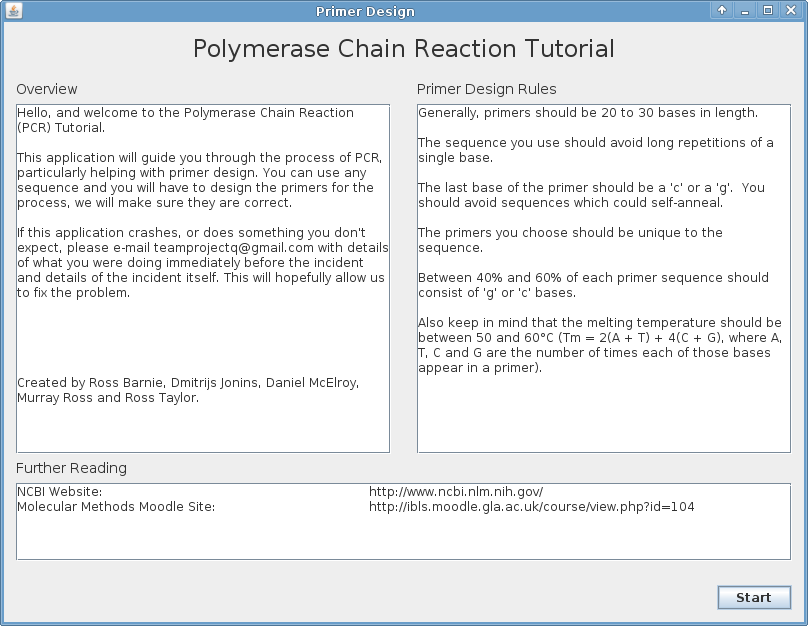
\includegraphics[width=0.6\textwidth]{./images/demoBuild/splash.png}
    \caption{
      \label{fig:demoBuild:splash}
      Demo Build, Overview Panel 
    }
  \end{center}
\end{figure}

\paragraph{Sequence Entry}

\begin{figure}[h]
  \begin{center}
    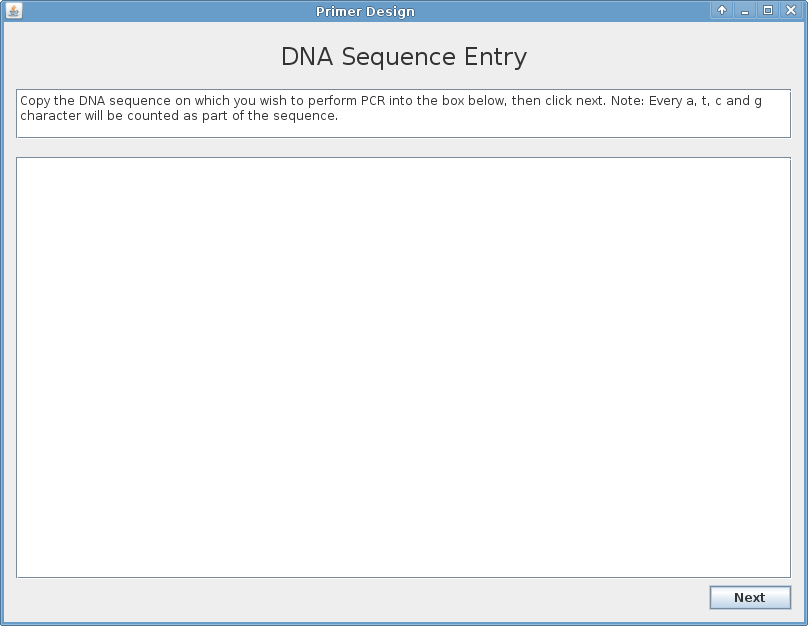
\includegraphics[width=0.6\textwidth]{./images/demoBuild/sequenceEntry.png}
    \caption{
      \label{fig:demoBuild:sequenceEntry}
      Demo Build, sequence entry panel 
    }
  \end{center}
\end{figure}

Figure \ref{fig:demoBuild:sequenceEntry} shows the next panel,
referred to by the team as the ``sequence entry'' panel.
While based on the design discussed in section \ref{design:ui} it
has been altered slightly to maximise the amount of space to be used
for entering in the sequence, as this is the primary purpose of this
panel.

It was expected of the user to go to the National Center for
Biotechnology Information (NCBI) website and obtain a DNA sequence by
copying it to their clipboard and then pasting this into the sequence
entry panel and this was explained in the accompanying user guide
(appendix \ref{app:userGuideDemo}).
Although this relied heavily on the users' ability to use keyboard
shortcuts, it was assumed that all students at university level would
at least have an awareness of these shortcuts.
We also assumed that once students were told of these shortcuts, as
they were in the user guide, that they would be comfortable using
them.

%---------------------------------------------------------------------

\paragraph{Target Selection}

\begin{figure}[h]
  \begin{center}
    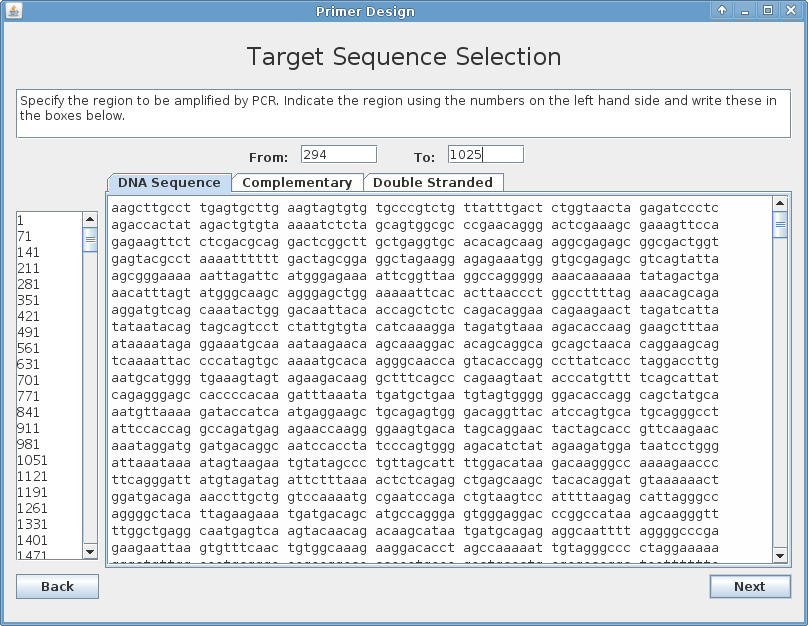
\includegraphics[width=0.6\textwidth]{./images/demoBuild/areaSelection.png}
    \caption{
      \label{fig:demoBuild:areaSelection}
      Demo Build, Area Selection Panel
    }
  \end{center}
\end{figure}

Following the Sequence Entry panel is the ``Area Selection'' or
``Target Selection'' panel, seen in figure
\ref{fig:demoBuild:areaSelection}, which requires the user to specify
the ``target'' sequence, ie the desired output sequence of the PCR
process.
This is accomplished by the user entering the start of the sequence
that they want and the end of the sequence they want, both by the
index of that base in the sequence, into the ``From'' and ``To''
fields at the bottom of the panel.

This would, ideally, be helped by the text pane at the left of the
screen which shows the base number of the first base on its line.
Unfortunately, for an unknown reason, the text panes became misaligned
when viewed from any platform other than the one we were using for
development (the level 3 Computing Science Laboratory computers
running Scientific Linux) and this misalignment can be seen in figure
\ref{fig:demoBuild:areaSelection}.

An addition made to the original design discussed in section
\ref{design:ui} is the tabs above the main text area, which allow the
user to switch between the sequence they entered, and its
complementary equivalent, generated by the program
It was a suggestion by the clients to have this feature as it would
greatly increase the speed at which the user could design the reverse
primer.
Without the complementary tab, not only would the user have to
manually convert the primer to its complementary equivalent, but also
reverse its order, which neither the team or the clients felt was a
useful way for students to spend their time. 

%---------------------------------------------------------------------

\paragraph{Primer Design}

Following the Area Selection panel is the ``Primer Design'' panel,
shown in figure \ref{fig:demoBuild:primerDesign}, which allows the
user to enter forward and reverse primers.

\begin{figure}[h]
  \begin{center}
    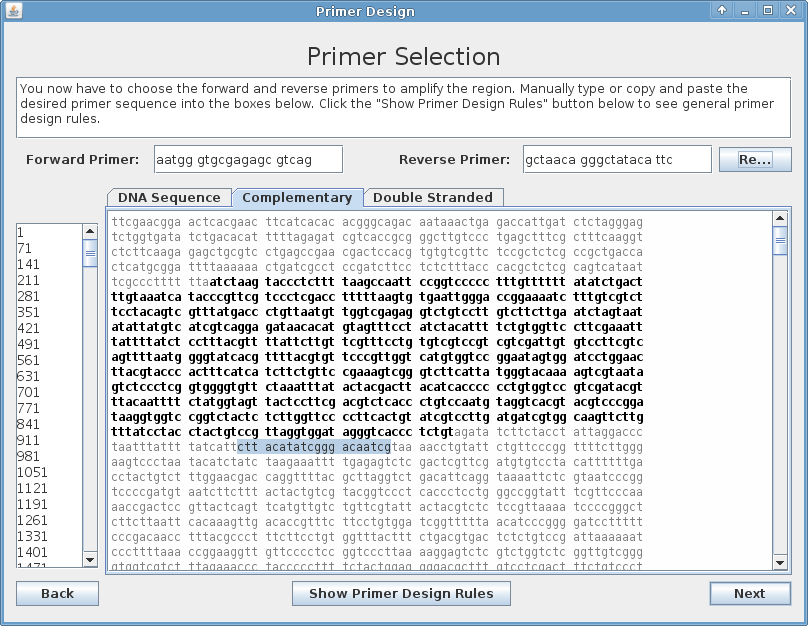
\includegraphics[width=0.6\textwidth]{./images/demoBuild/primerDesign.png}
    \caption{
      \label{fig:demoBuild:primerDesign}
      Demo Build, Primer Design Panel
    }
  \end{center}
\end{figure}

One of the design features we had intended to provide was ``dynamic
highlighting'', as it was referred to by the team, which was going to
provide a highlight around what the user enters into the primer text
fields.
This highlighting was unfortunately missing in the demo build due to
time constraints.

However, we had always intended to give feedback to the user should
they break rules of primer design and the demo build version of this
can be seen in figure \ref{fig:demoBuild:primerFeedback} and appears
when the user clicks the ``Next'' button.
Again based on the design (section \ref{design:ui}), this dialogue
window shows the user any rules which they have broken, and which
primer the feedback is referring to.

\begin{figure}[h]
  \begin{center}
    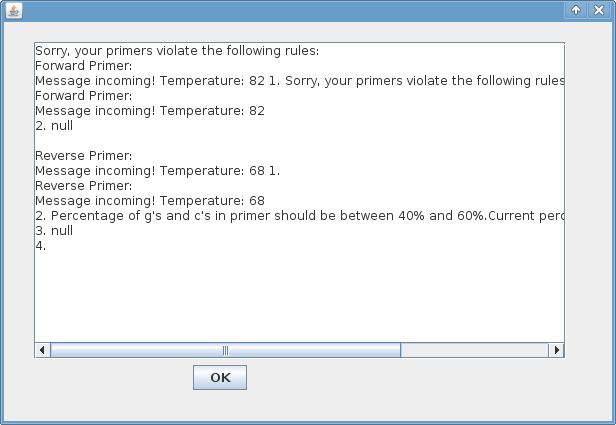
\includegraphics[width=0.6\textwidth]{./images/demoBuild/primerFeedback.png}
    \caption{
      \label{fig:demoBuild:primerFeedback}
      Demo Build, Feedback on User-entered Primer
    }
  \end{center}
\end{figure}

Again, due to time constraints this was not as fully featured as we
had hoped for in the demonstration, however it did display enough
information to give an idea to our clients of what the feedback might
look like in the future (see further discussion in section
\ref{eval:demo}).

In order to design a reverse primer outwith the system, the
complementary strand would have to be calculated (which would be in
the 3'---5' direction) and reversed to be in the correct direction
(5'---3').
In the application, the complementary strand is already calculated, so
the user can simply copy and paste a primer of their choosing from the
sequence and put it in the reverse primer text field.
However, this does not solve the problem of reversing it, so the
``Reverse'' button was put next to the reverse primer text field,
which, intuitively, reverses the order of the primer in the text
field. 

At the bottom of the panel in the middle of the ``Back'' and ``Next''
buttons is the ``Primer Design Rules'' button, which shows,
intuitively enough, the primer design rules set out at the beginning
of the program.
This was part of the initial design, the button for which can be seen
in figure \ref{fig:uiDes:slide3} and the implementation of which can
be seen in figure \ref{fig:demoBuild:primerDesignRules}.

\begin{figure}[h]
  \begin{center}
    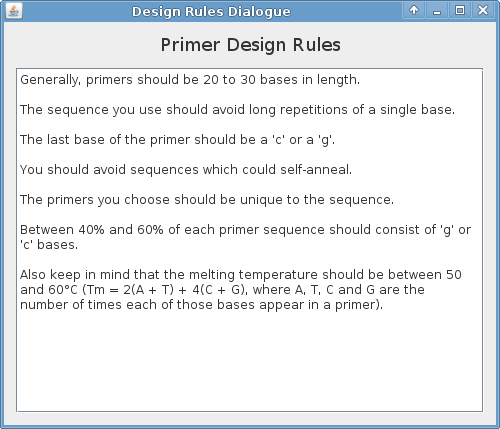
\includegraphics[width=0.6\textwidth]{./images/demoBuild/primerDesignRules.png}
    \caption{
      \label{fig:demoBuild:primerDesignRules}
      Demo Build, Primer Design Rules Dialogue
    }
  \end{center}
\end{figure}

\paragraph{Melting Temperature}

After designing a primer, the user is presented with the ``Melting
Temperature'' panel as seen in figure \ref{fig:demoBuild:meltingTemp}
for the user to evaluate their primers.

In the case of the demonstration, this panel was blocked from the user
unless they had a correct primer.

\begin{figure}[h]
  \begin{center}
    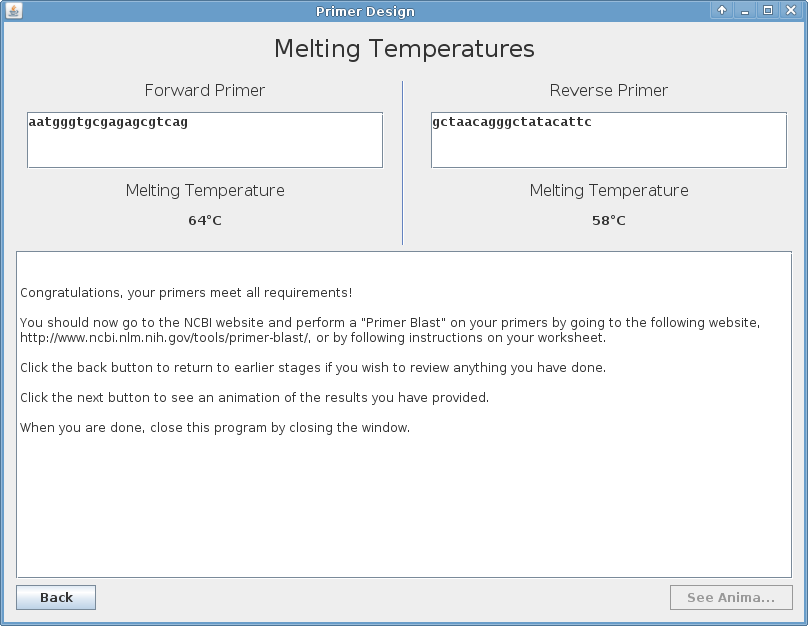
\includegraphics[width=0.6\textwidth]{./images/demoBuild/meltingTemp.png}
    \caption{
      \label{fig:demoBuild:meltingTemp}
      Demo Build, Melting Temperatures of User's Primers.
    }
  \end{center}
\end{figure}

In terms of design, the initial design proved to be near-impossible to
reproduce in Swing and make it look professional and after several
iterations became what it is.
The emphasis on the primers and the melting temperatures in bold means
that the user can easily see their primers and the associated melting
temperatures, while the separator down the center visually separates
the forward from the reverse primer.

Unfortunately the animation was not available in time for the
demonstration and although the button for it was included in this
panel it was disabled.

%---------------------------------------------------------------------

\subsubsection{Current Build}

Addressing feedback from the demonstration (see section \ref{eval:demo}),
and adding new elements to provide extra functionality, the current
build is several iterations ahead of the demo build discussed above
and is currently available to all Molecular Methods students.

While there have been many changes to the build in this time, not much
has been changed in terms of the UI as most feedback about it at the
demonstration was positive.
Most changes stem from either additional requirements or from the
demonstration feedback.

\paragraph{Overview}
The overview screen (seen in figure \ref{fig:demoBuild:splash})
changed only because of the addition of the menu bar, discussed
below.
It was felt that this needed very little change, if any, from the demo
build and is therefore the same as the demo build version in almost
every respect.

\paragraph{Sequence Entry}

\begin{figure}[h]
  \begin{center}
    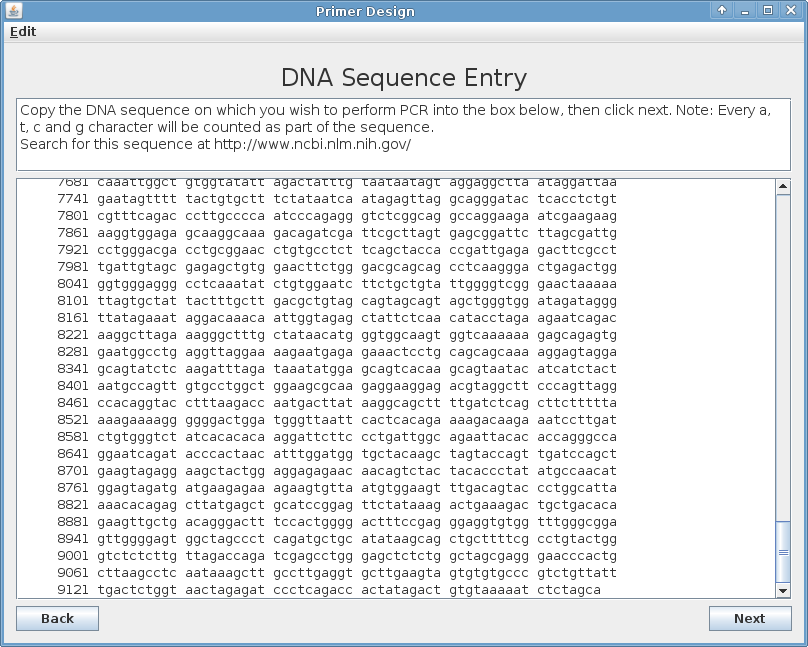
\includegraphics[width=0.6\textwidth]{./images/currentBuild/sequenceEntry.png}
    \caption{
      \label{fig:currentBuild:sequenceEntry}
      Current Build, Sequence Entry Panel
    }
  \end{center}
\end{figure}

In terms of changes made after the demo build, this panel is similar
to the Overview panel above in that neither have been changed to any
significant degree.

Though, as can be seen in figure \ref{fig:currentBuild:sequenceEntry}
there have been some minor changes.

Firstly, the menu bar at the top of the panel, which was added to
address the issue of people not being familiar with keyboard
shortcuts.
The menu itself was named ``Edit'' to conform to standards set by most
applications with menu bars in that the ``Copy'' and ``Paste''
features are usually found under the ``Edit'' menu.

Lastly, the ``Back'' button on this panel which was not present for
the demo build.
For the demo build, it felt unnecessary to have a back button since
any information that people would actually need to use the program is
available throughout the application (ie Primer Design Rules is
available on Primer Design panel, NCBI website is given to user in the
instructions at top of panel).
However, the clients asked that we put the ``Back'' button in.

\paragraph{Target Selection}

\begin{figure}[h]
  \begin{center}
    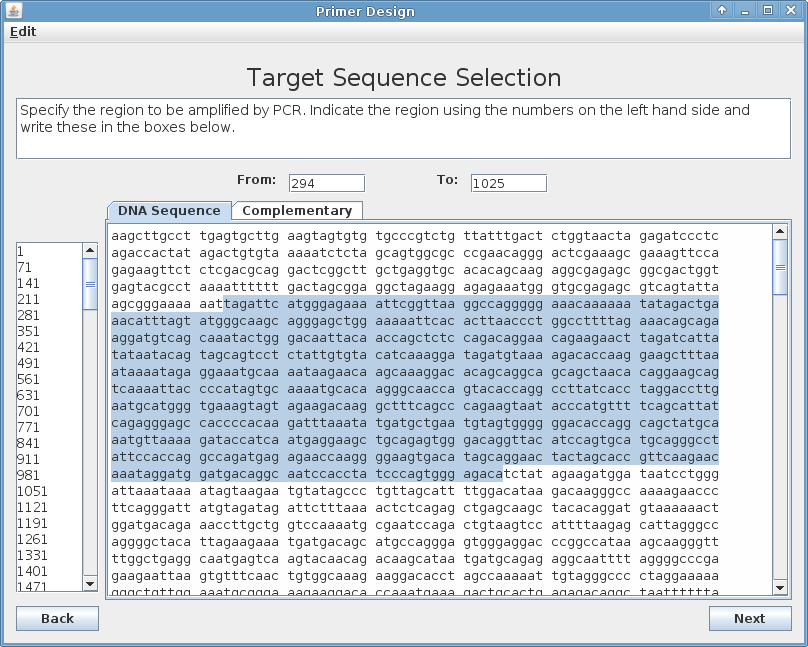
\includegraphics[width=0.6\textwidth]{./images/currentBuild/areaSelection.png}
    \caption{
      \label{fig:currentBuild:areaSelection}
      Current Build, Target Selection Panel
    }
  \end{center}
\end{figure}

While the interface of the Target Selection panel may not have changed
(much) from the demo build, the way a user pulls their desired
sequence has changed to make the process much easier.

Previously, as discussed in section \ref{fig:demoBuild:areaSelection},
the user would have to find the indexes of the start and end of the
sequence they wanted to copy.
Now, as can be seen in figure \ref{fig:currentBuild:areaSelection},
the user simply has to highlight the desired sequence and the indexes
are calculated automatically.
This change means that users do not have to depend on the unreliable
line numbers, and can focus instead on the actual sequence.
It also provides a visual way of seeing where your sequence is,
without having to switch between this and the next panel, which was
one of the issues brought up in the demonstration (see section
\ref{eval:demo}).

\paragraph{Primer Design}

\begin{figure}[h]
  \begin{center}
    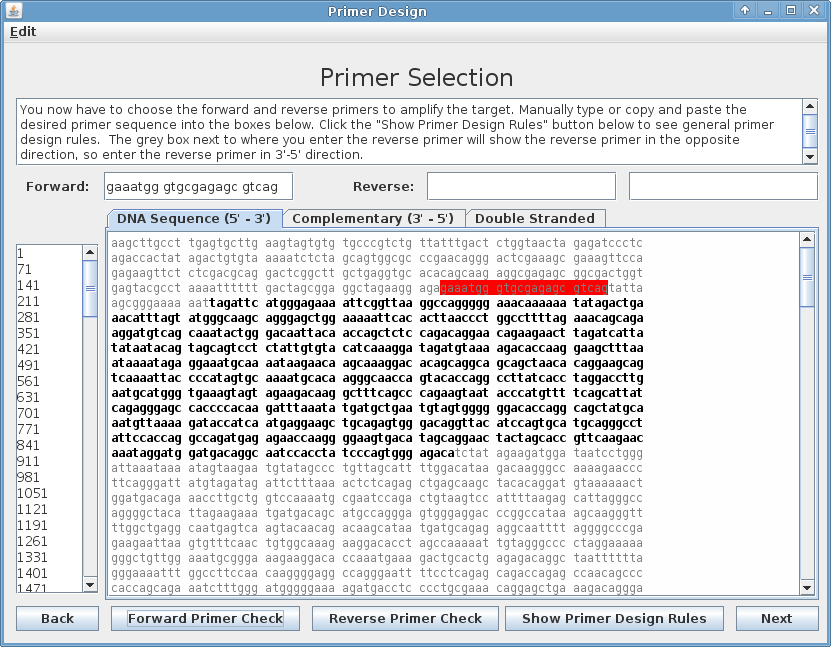
\includegraphics[width=0.6\textwidth]{./images/currentBuild/forwardPrimerDesignRed.png}
    \caption{
      \label{fig:currentBuild:forwardPrimerDesignRed}
      Current Build, (Forward) Primer Design, showing invalid primer selection
    }
  \end{center}
\end{figure}

Primer design received a lot of attention in that it received the
majority of new features in the application since the demo build.

Firstly, a feature referred to by the team as ``dynamic highlighting''
which, when a user types in a sequence to the primer text fields,
highlights that sequence within the whole sequence and this can be
seen in figure \ref{fig:currentBuild:forwardPrimerDesignRed}.
Initially, this highlighting was going to be a single colour simply to
help the user see if the primer is unique to the sequence, and so that
they can visualise where the primer is within the sequence.
The lack of visual aids in the demo build was something we strove to
rectify especially after the feedback from the demonstration (section
\ref{eval:demo}).
To this end we also made the highlight change colour depending on the
correctness of the primer, how this is decided is discussed in section
\ref{impl:models:dynHigh}.
This can be seen in figure
\ref{fig:currentBuild:forwardPrimerDesignRed} with an incorrect
primer, and figure \ref{fig:currentBuild:forwardPerfectPrimer} with a
perfect primer.

\begin{figure}[h]
  \begin{center}
    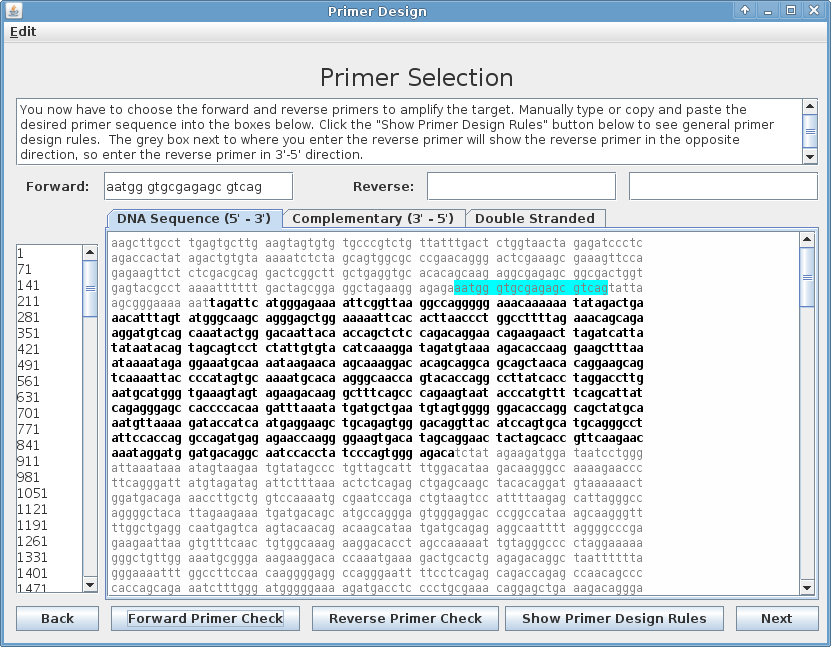
\includegraphics[width=0.6\textwidth]{./images/currentBuild/forwardPerfectPrimer.png}
    \caption{
      \label{fig:currentBuild:forwardPerfectPrimer}
      Current Build, (Forward) Primer Design, showing perfect primer selection
    }
  \end{center}
\end{figure}

Another new feature added based on the demonstration feedback was the
two new buttons at the bottom of the panel, which give feedback on a
single primer, depending on which button the user presses.
An example of what that feedback looks like can be seen in figure
\ref{fig:currentBuild:primerEvalRed}.

\begin{figure}[h]
  \begin{center}
    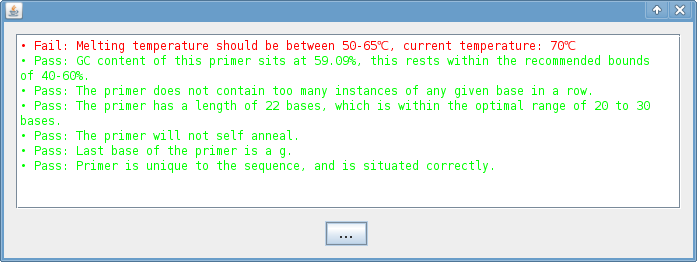
\includegraphics[width=0.6\textwidth]{./images/currentBuild/primerEvalRed.png}
    \caption{
      \label{fig:currentBuild:primerEvalRed}
      Current Build, Single Primer Feedback
    }
  \end{center}
\end{figure}

This feedback is also colour-coded to make any problems with the
user's primer(s) more immediately apparent than in the demo build.

With the emphasis on direction of the sequence being made more obvious
in this version with the direction shown in the tab names, it is more
obvious as to which direction the user should be thinking about when
creating the reverse primer.
To allow the user to only have to think about one direction, the
``Reverse'' button from the demo build was replaced by an uneditable
text field which auto-generates the reverse order of the reverse
primer, see figure \ref{fig:currentBuild:reversePrimerPerfect}.

\begin{figure}[h]
  \begin{center}
    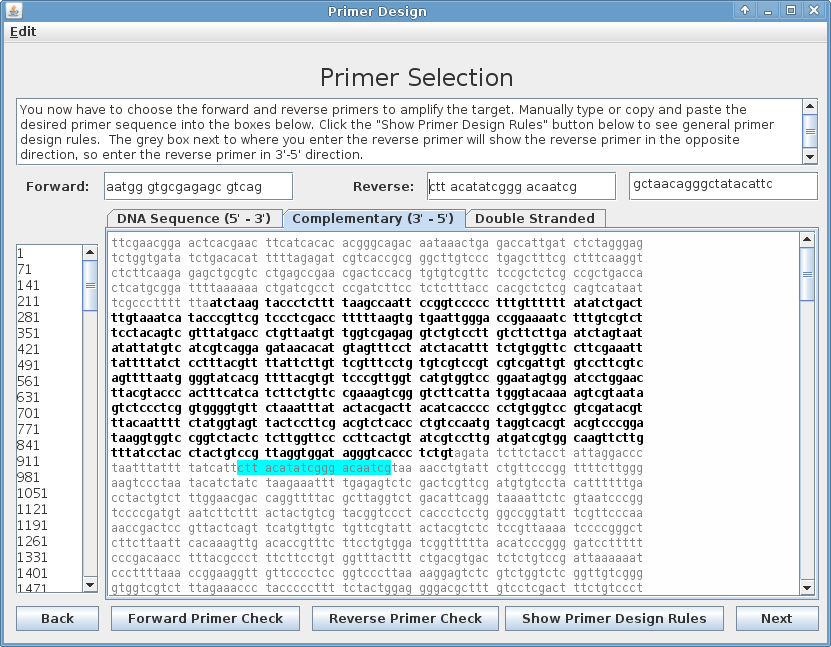
\includegraphics[width=0.6\textwidth]{./images/currentBuild/reversePrimerPerfect.png}
    \caption{
      \label{fig:currentBuild:reversePrimerPerfect}
      Current Build, Reverse Primer (showing perfect primer)
    }
  \end{center}
\end{figure}

When the user presses the ``Next'' button, they are presented with a
dialogue box, giving a list of all the passed, failed and
``close-fail''-ed rules for the primers individually and the more
general rules (see figure \ref{fig:currentBuild:primerDesignBothFeedback}.
Again, these are colour-coded.

\begin{figure}[h]
  \begin{center}
    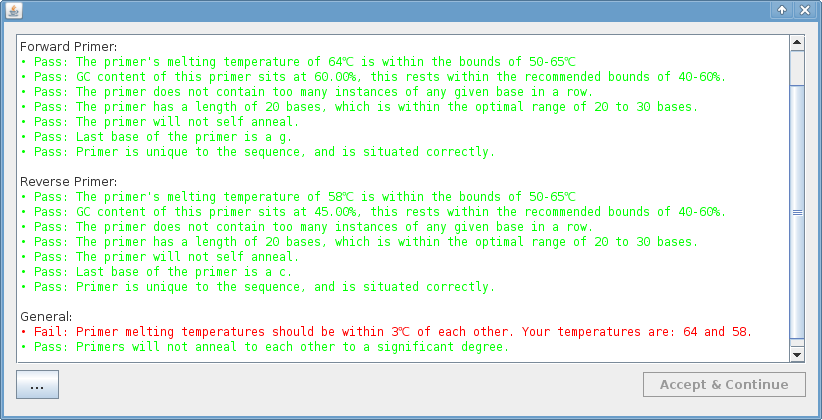
\includegraphics[width=0.6\textwidth]{./images/currentBuild/primerDesignBothFeedback.png}
    \caption{
      \label{fig:currentBuild:primerDesignBothFeedback}
      Current Build, Feedback on both primers dialogue
    }
  \end{center}
\end{figure}

